% Options for packages loaded elsewhere
\PassOptionsToPackage{unicode}{hyperref}
\PassOptionsToPackage{hyphens}{url}
%
\documentclass[
]{article}
\usepackage{lmodern}
\usepackage{amsmath}
\usepackage{ifxetex,ifluatex}
\ifnum 0\ifxetex 1\fi\ifluatex 1\fi=0 % if pdftex
  \usepackage[T1]{fontenc}
  \usepackage[utf8]{inputenc}
  \usepackage{textcomp} % provide euro and other symbols
  \usepackage{amssymb}
\else % if luatex or xetex
  \usepackage{unicode-math}
  \defaultfontfeatures{Scale=MatchLowercase}
  \defaultfontfeatures[\rmfamily]{Ligatures=TeX,Scale=1}
\fi
% Use upquote if available, for straight quotes in verbatim environments
\IfFileExists{upquote.sty}{\usepackage{upquote}}{}
\IfFileExists{microtype.sty}{% use microtype if available
  \usepackage[]{microtype}
  \UseMicrotypeSet[protrusion]{basicmath} % disable protrusion for tt fonts
}{}
\makeatletter
\@ifundefined{KOMAClassName}{% if non-KOMA class
  \IfFileExists{parskip.sty}{%
    \usepackage{parskip}
  }{% else
    \setlength{\parindent}{0pt}
    \setlength{\parskip}{6pt plus 2pt minus 1pt}}
}{% if KOMA class
  \KOMAoptions{parskip=half}}
\makeatother
\usepackage{xcolor}
\IfFileExists{xurl.sty}{\usepackage{xurl}}{} % add URL line breaks if available
\IfFileExists{bookmark.sty}{\usepackage{bookmark}}{\usepackage{hyperref}}
\hypersetup{
  pdftitle={Computational calculation and visualization of the Biological Value Index},
  pdfauthor={Juan Carlos Villaseñor-Derbez; Ricardo Dominguez-Reza; Los que falten},
  hidelinks,
  pdfcreator={LaTeX via pandoc}}
\urlstyle{same} % disable monospaced font for URLs
\usepackage[margin=1in]{geometry}
\usepackage{longtable,booktabs}
\usepackage{calc} % for calculating minipage widths
% Correct order of tables after \paragraph or \subparagraph
\usepackage{etoolbox}
\makeatletter
\patchcmd\longtable{\par}{\if@noskipsec\mbox{}\fi\par}{}{}
\makeatother
% Allow footnotes in longtable head/foot
\IfFileExists{footnotehyper.sty}{\usepackage{footnotehyper}}{\usepackage{footnote}}
\makesavenoteenv{longtable}
\usepackage{graphicx}
\makeatletter
\def\maxwidth{\ifdim\Gin@nat@width>\linewidth\linewidth\else\Gin@nat@width\fi}
\def\maxheight{\ifdim\Gin@nat@height>\textheight\textheight\else\Gin@nat@height\fi}
\makeatother
% Scale images if necessary, so that they will not overflow the page
% margins by default, and it is still possible to overwrite the defaults
% using explicit options in \includegraphics[width, height, ...]{}
\setkeys{Gin}{width=\maxwidth,height=\maxheight,keepaspectratio}
% Set default figure placement to htbp
\makeatletter
\def\fps@figure{htbp}
\makeatother
\setlength{\emergencystretch}{3em} % prevent overfull lines
\providecommand{\tightlist}{%
  \setlength{\itemsep}{0pt}\setlength{\parskip}{0pt}}
\setcounter{secnumdepth}{5}
\usepackage{booktabs}
\usepackage{longtable}
\usepackage{array}
\usepackage{multirow}
\usepackage{wrapfig}
\usepackage{float}
\usepackage{colortbl}
\usepackage{pdflscape}
\usepackage{tabu}
\usepackage{threeparttable}
\usepackage{threeparttablex}
\usepackage[normalem]{ulem}
\usepackage{makecell}
\usepackage{xcolor}
\ifluatex
  \usepackage{selnolig}  % disable illegal ligatures
\fi
\newlength{\cslhangindent}
\setlength{\cslhangindent}{1.5em}
\newlength{\csllabelwidth}
\setlength{\csllabelwidth}{3em}
\newenvironment{CSLReferences}[2] % #1 hanging-ident, #2 entry spacing
 {% don't indent paragraphs
  \setlength{\parindent}{0pt}
  % turn on hanging indent if param 1 is 1
  \ifodd #1 \everypar{\setlength{\hangindent}{\cslhangindent}}\ignorespaces\fi
  % set entry spacing
  \ifnum #2 > 0
  \setlength{\parskip}{#2\baselineskip}
  \fi
 }%
 {}
\usepackage{calc}
\newcommand{\CSLBlock}[1]{#1\hfill\break}
\newcommand{\CSLLeftMargin}[1]{\parbox[t]{\csllabelwidth}{#1}}
\newcommand{\CSLRightInline}[1]{\parbox[t]{\linewidth - \csllabelwidth}{#1}\break}
\newcommand{\CSLIndent}[1]{\hspace{\cslhangindent}#1}

\title{Computational calculation and visualization of the Biological Value Index}
\author{Juan Carlos Villaseñor-Derbez\footnote{Bren School, \href{mailto:john@example.org}{\nolinkurl{john@example.org}}} \and Ricardo Dominguez-Reza\footnote{CICESE, \href{mailto:jane@example.org}{\nolinkurl{jane@example.org}}} \and Los que falten}
\date{}

\begin{document}
\maketitle
\begin{abstract}
Abstract goes here
\end{abstract}

{
\setcounter{tocdepth}{2}
\tableofcontents
}
\#Introduction

Todo esto es mierda, tengo que modificarlo

\begin{itemize}
\tightlist
\item
  Indices in ecology
\end{itemize}

Usually people describe a site by the species that inhabit it, but do not pay much attention to how some species are incharged of the simmilarities.

\begin{itemize}
\item
  History of the index
  - When it was proposed
  - How it worked
  - Modifications by Loya Salinas
  - How it works now
\item
  Usage of the index
  - Works that have used it
\item
  Stating the problem

  \begin{itemize}
  \tightlist
  \item
    Lack of comparison
  \item
    computability
  \end{itemize}
\end{itemize}

\hypertarget{materials-and-methods}{%
\section{Materials and Methods}\label{materials-and-methods}}

\begin{itemize}
\item
  How the index works, step by step (possibly citing Loya-Salinas)
\item
  Flow diagram depfun(ivb)
\item
  Adding the \%BVI
\end{itemize}

\begin{equation}\%BVI_i = \frac{(100\times BVI_i)}{\sum_{i = 1}^nBVI_i}\end{equation}

\begin{itemize}
\item
  Compare N and Ni vs rBVI to test its usefulness
\item
  Propose ways to visualize rBVI
\item
  Recreating Loya-Salinas
\end{itemize}

\begin{tabular}{>{}lrrrrrr}
\toprule
Spp & S1 & S2 & S3 & S4 & S5 & S6\\
\midrule
\em{Synchelidium spp.} & 2398 & 1626 & 811 & 1275 & 1343 & 7079\\
\em{Tridentella spp.} & 2048 & 1125 & 528 & 1990 & 1098 & 1274\\
\em{Nerine cirratulus} & 37 & 165 & 1141 & 1540 & 118 & 53\\
\em{Nephtys californiensis} & 544 & 875 & 404 & 170 & 58 & 90\\
\em{Glycera tenuis} & 265 & 566 & 106 & 646 & 133 & 118\\
\addlinespace
\em{Donax gouldii} & 914 & 75 & 42 & 5 & 5 & 15\\
\em{Orchestoidea benedicti} & 11 & 251 & 133 & 79 & 162 & 245\\
\em{Archaeomysis spp.} & 958 & 90 & 160 & 37 & 522 & 111\\
\em{Armadillium spp.} & 59 & 155 & 91 & 16 & 208 & 283\\
\em{Megalopus spp.} & 149 & 266 & 48 & 30 & 0 & 0\\
\addlinespace
\em{Emerita analoga} & 101 & 16 & 96 & 27 & 0 & 10\\
\em{Pontharpinia spp.} & 69 & 96 & 11 & 16 & 0 & 0\\
\em{Euzonus mucronata} & 0 & 0 & 37 & 341 & 0 & 0\\
\em{Lepidopa californica} & 5 & 69 & 16 & 0 & 16 & 0\\
\em{Magelona californica} & 0 & 5 & 5 & 0 & 42 & 10\\
\addlinespace
\em{Hanstorina spp.} & 0 & 16 & 5 & 0 & 0 & 0\\
\em{Glycera dibranchiata} & 0 & 0 & 0 & 0 & 5 & 0\\
\em{Archaeomysis maculata} & 0 & 0 & 0 & 5 & 0 & 0\\
\bottomrule
\end{tabular}

\begin{itemize}
\tightlist
\item
  Mention using SIMPER as a comparative
\item
  Propose a graph to visualize data
\end{itemize}

\hypertarget{results}{%
\section{Results}\label{results}}

\begin{itemize}
\tightlist
\item
  Results from Loya-Salinas
\item
  Graph
\item
  Comparing \%BVI with SIMPER
\item
  Table with abundances, BVI, \%BVI and SIMPER
\end{itemize}

\begin{tabular}{>{}lllllllllr}
\toprule
  & Species & S1 & S2 & S3 & S4 & S5 & S6 & BVI & \%BVI\\
\midrule
\em{Synchelidium spp.} & Synchelidium spp. & 10 & 10 & 9 & 8 & 10 & 10 & 57 & 17.22\\
\em{Tridentella spp.} & Tridentella spp. & 9 & 9 & 8 & 10 & 9 & 9 & 54 & 16.31\\
\em{Glycera tenuis} & Glycera tenuis & 5 & 7 & 4 & 7 & 5 & 6 & 34 & 10.27\\
\em{Nephtys californiensis} & Nephtys californiensis & 6 & 8 & 7 & 5 & 3 & 4 & 33 & 9.97\\
\em{Archaeomysis spp.} & Archaeomysis spp. & 8 & 1 & 6 & 3 & 8 & 5 & 31 & 9.37\\
\addlinespace
\em{Nerine cirratulus} & Nerine cirratulus & 0 & 4 & 10 & 9 & 4 & 3 & 30 & 9.06\\
\em{Orchestoidea benedicti} & Orchestoidea benedicti & 0 & 5 & 5 & 4 & 6 & 7 & 27 & 8.16\\
\em{Armadillium spp.} & Armadillium spp. & 1 & 3 & 2 & 0 & 7 & 8 & 21 & 6.34\\
\em{Megalopus spp.} & Megalopus spp. & 4 & 6 & 1 & 2 & 0 & 0 & 13 & 3.93\\
\em{Donax gouldii} & Donax gouldii & 7 & 0 & 0 & 0 & 0 & 2 & 9 & 2.72\\
\addlinespace
\em{11} & Others & 5 & 2 & 3 & 7 & 3 & 2 & 22 & 0.07\\
\em{1} & Total &  &  &  &  &  &  &  & 100.00\\
\bottomrule
\end{tabular}

\begin{table}[!htbp] \centering 
  \caption{} 
  \label{} 
\begin{tabular}{@{\extracolsep{5pt}}lcc} 
\\[-1.8ex]\hline 
\hline \\[-1.8ex] 
 & \multicolumn{2}{c}{\textit{Dependent variable:}} \\ 
\cline{2-3} 
\\[-1.8ex] & %N & log10(n) \\ 
\\[-1.8ex] & (1) & (2)\\ 
\hline \\[-1.8ex] 
 rBVI & 0.016$^{***}$ (0.002) & 0.118$^{***}$ (0.010) \\ 
  Constant & $-$0.040$^{**}$ (0.016) & 1.189$^{***}$ (0.090) \\ 
 \hline \\[-1.8ex] 
Observations & 81 & 81 \\ 
R$^{2}$ & 0.489 & 0.636 \\ 
Residual Std. Error (df = 79) & 0.088 & 0.482 \\ 
F Statistic (df = 1; 79) & 75.486$^{***}$ & 138.264$^{***}$ \\ 
\hline 
\hline \\[-1.8ex] 
\textit{Note:}  & \multicolumn{2}{r}{$^{*}$p$<$0.1; $^{**}$p$<$0.05; $^{***}$p$<$0.01} \\ 
\end{tabular} 
\end{table}

\clearpage

\begin{verbatim}
## `geom_smooth()` using formula 'y ~ x'
## `geom_smooth()` using formula 'y ~ x'
\end{verbatim}

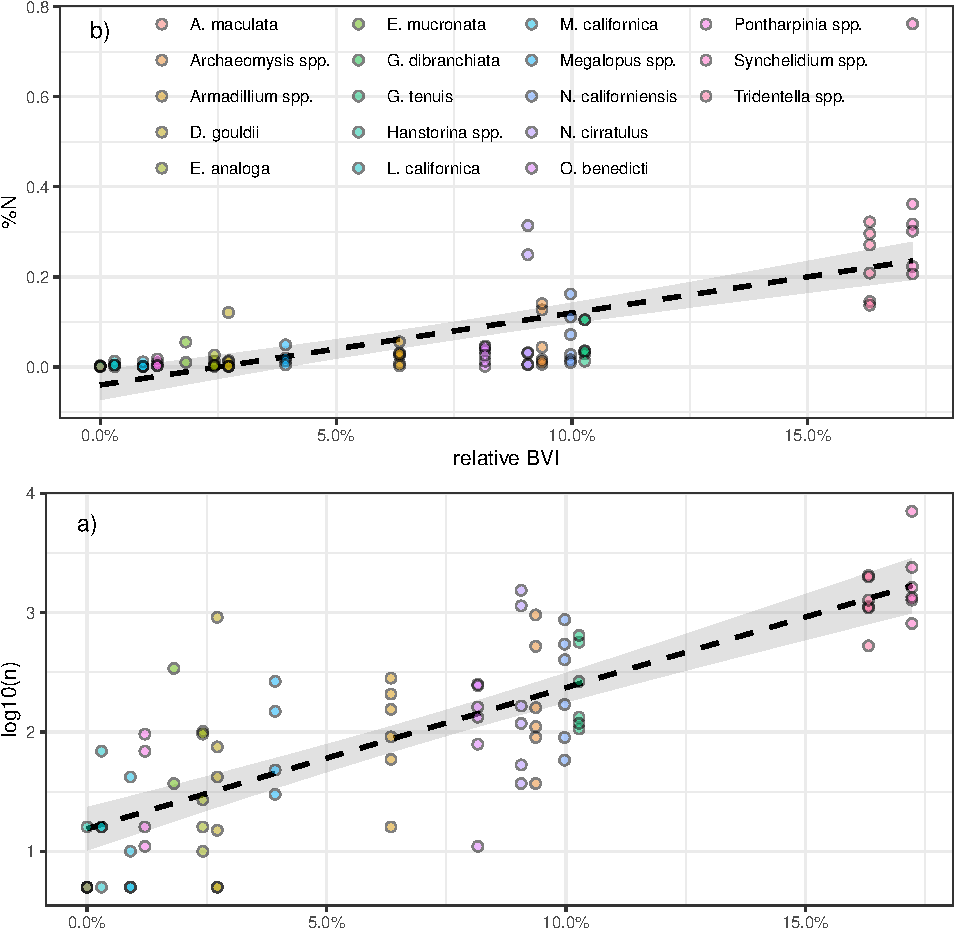
\includegraphics{manuscript_files/figure-latex/unnamed-chunk-7-1.pdf}

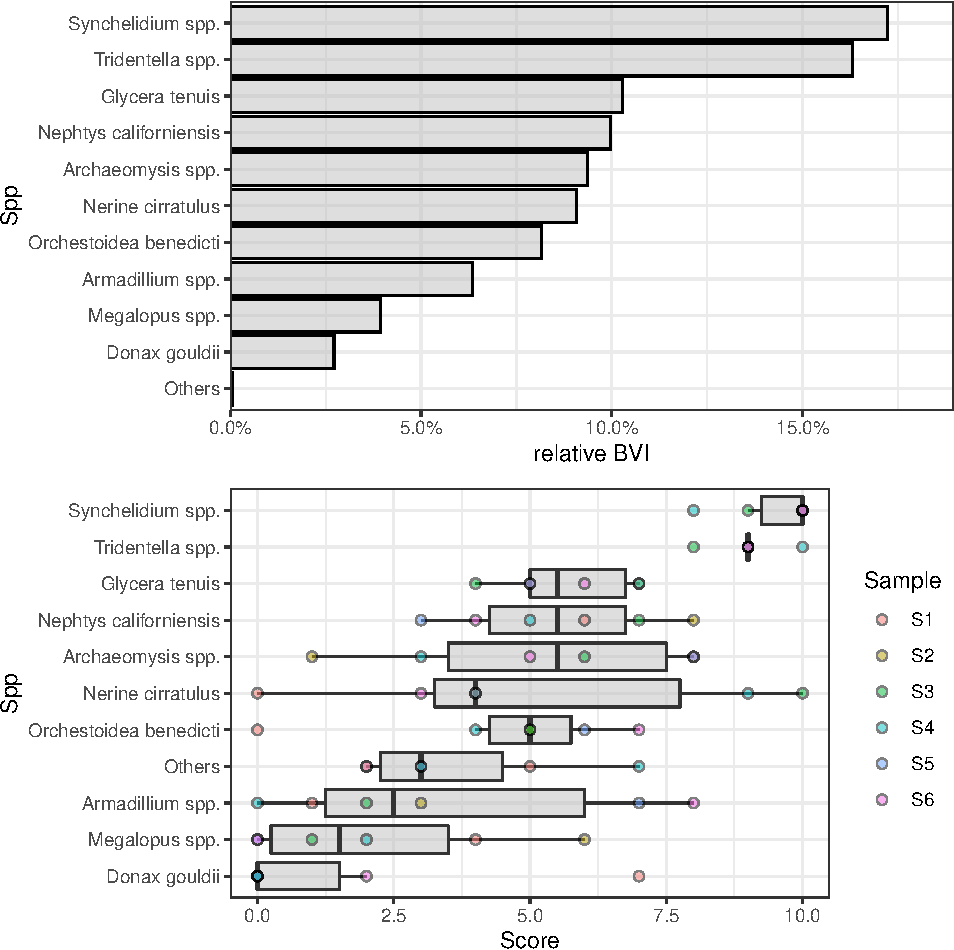
\includegraphics{manuscript_files/figure-latex/unnamed-chunk-8-1.pdf}

\hypertarget{discussion-and-conclusions}{%
\section{Discussion and Conclusions}\label{discussion-and-conclusions}}

\hypertarget{references}{%
\section{References}\label{references}}

\hypertarget{refs}{}
\begin{CSLReferences}{0}{0}
\end{CSLReferences}

\hypertarget{figures-and-tables}{%
\section{Figures and Tables}\label{figures-and-tables}}

\end{document}
